\documentclass[rinkou,a4paper]{ieicej}
% \usepackage{graphicx}
\usepackage[dvipdfmx]{graphicx}
\usepackage{url}
\usepackage{paralist}
\usepackage{nidanfloat}
\usepackage{ascmac}
\usepackage{fancybox}
\usepackage{amsmath}
\usepackage{breqn}
\usepackage{amssymb}
\usepackage{amsfonts}
\usepackage{pifont}
\usepackage{multirow}
\usepackage{comment}

% UserSetting
\newenvironment{narrow}{\baselineskip=3mm}

\setcounter{page}{1}
\vol{103}%year
\no{05}%month
\day{12}%day

\jtitle{HTTP通信におけるIPv4とIPv6のネットワーク環境比較}%title
\jsubtitle
\authorlist{
 \authorentry{平野 紘大}{Kodai HIRANO}{}
} \vspace{-3mm}
\begin{document}

\maketitle

\section{はじめに}
本日の輪講では,私が取り組んでいるネットワーク計測に関する研究の進捗を報告する.
\ref{sec:explain}章で,今回使用するオープンソースの計測プログラムについて説明する.

\section{オープンソースによる計測}\label{sec:explain}
オープンソース(https:\slash\slash{}github.com\slash{}librespeed\slash{}speedtest)を用いて計測を行う.
サーバーはApache2によって動いている.
テストはIPアドレスの情報の取得,Pingテスト,Downloadテスト,Uploadテストの順に行う.それぞれ,以下のような実装になっている.

\subsection{IPアドレスに関する情報の取得}
サーバーにXMLHttpRequestでGETする.サーバーはipinfo.io(https:\slash\slash{}ipinfo.io)から得られた情報を返す.

\subsection{Pingテスト}
サーバーは単に200を返す.PerformanceResourceTimingのresponseStartとrequestStartの差をRTTとする.10回計測し,RTTの最小値をPingとする.1つ前のRTTとの差をinstjitterとして
\[
  \begin{dmath}
    jitter = \begin{cases}
      jitter*0.3+instjitter*0.7&\\(instjitter>jitter)\\
      jitter*0.8+instjitter*0.2&\\(instjitter<=jitter)
    \end{cases}
  \end{dmath}
\]
をJitterとしている.

\subsection{Downloadテスト}
6つ並行で300ms毎に,サーバーにXMLHttpRequestでGETする.サーバーは100Mbyteの疑似ランダムなバイト文字列を返す.onloadedでリクエストを繰り返す.15秒で終了し,totLoaded[bit]\slash{}t[s]をdownload speedとしている.

\subsection{Uploadテスト}

\subsection{サーバーにポスト}

\section{}

\begin{figure}[p]
\centering
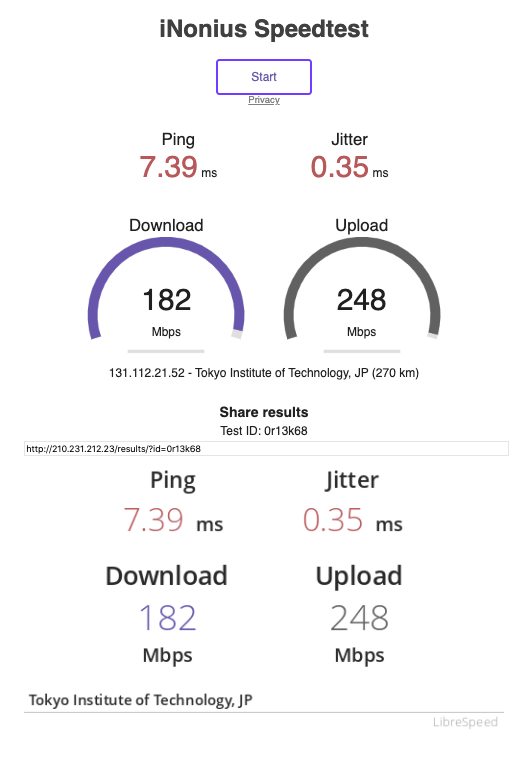
\includegraphics[scale = 0.3]{Screenshot.png}
\caption{現状のサイト(http://idaten.inonius.net/)}\label{ss}
\end{figure}

\begin{figure}[p]
\centering
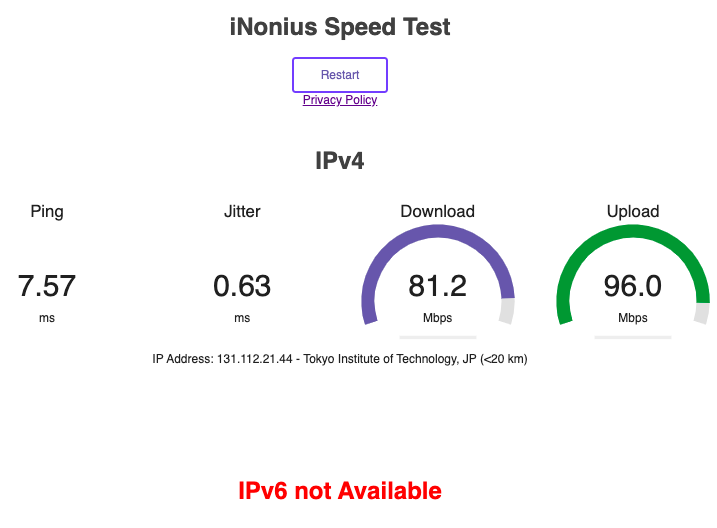
\includegraphics[scale = 0.3]{Screenshot2.png}
\caption{現状のサイト(IPv6がつながらない場合)}\label{ss}
\end{figure}

\begin{figure}[p]
\centering
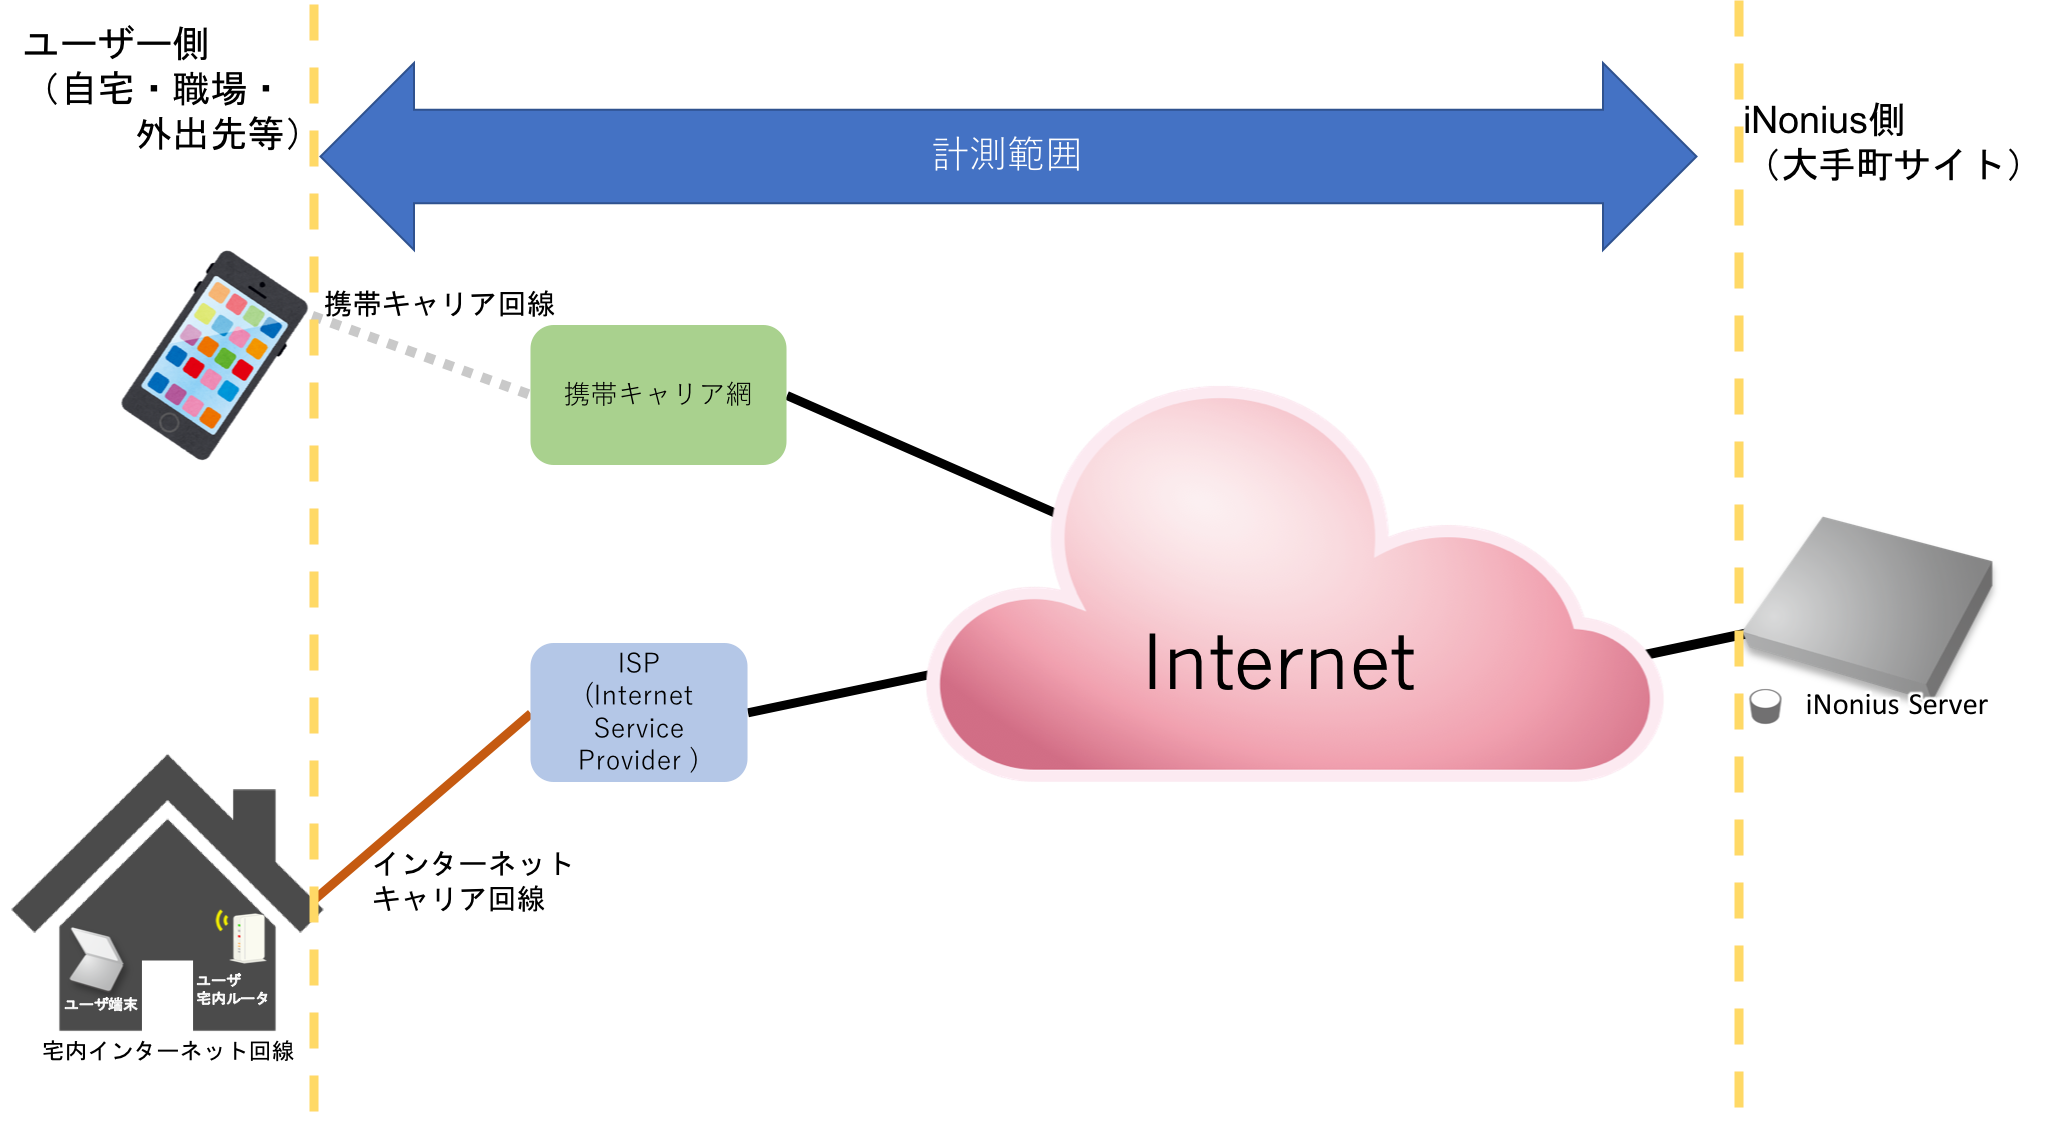
\includegraphics[scale = 0.25]{structure.png}
\caption{システム構成}\label{struct}
\end{figure}

\subsection{残タスク}
目標の計測環境を整えるための残タスクをまとめる.
\subsubsection{デュアルスタック}
サーバーをIPv4とIPv6の両方に対応させる.

また,IPv4の計測完了後,ユーザーのネットワークがIPv6に対応していた場合,可能であれば,自動的にIPv6での計測を始める.逆にIPv6の計測から始めた場合も同様に,自動的にIPv4での計測を始める
\subsubsection{ユーザー同定}
本研究の目的は,IPv4とIPv6の通信状況の比較である.したがって,同一のユーザーからのIPv4とIPv6の通信を比較,評価する必要がある.

北口らの研究\cite{kitaguchi1}では,urlパラメータに,userIdを持たせて,同じユーザーからの通信を識別している.これは\cite{kitaguchi2}でも利用されている.

また,大量のアクセスが同じユーザー(ヘビーユーザー)からあった場合,その影響を考慮する必要があるので,IPv4アドレスを基にユーザーを特定する.

また,Route Views Project\cite{routeview}が公開しているBGPのフルルート情報を用いて,AS情報を求める.

\subsubsection{PPPoEやIPoEなど通信路の形態の推定}
\cite{kitaguchi1}では,AS番号がIPv4とIPv6で異なるとき
\begin{itemize}
 \item IPv4とIPv6でそれぞれ別のAS経由でネイティブ接続している
 \item IPv4 over IPv6(IPv6はネイティブ)
\end{itemize}
のパターンは少ないと仮定し,IPv6はトンネル接続として,AS番号が同じならば,IPv6はネイティブであるとしている.

\cite{kitaguchi2}では,MSS値により,ヘッダの長さを求めて,通信路を推定している.また,[1]での推定方法との比較をして,上記の仮定を否定している.

本研究でも,MSSとTTLを計測したいと考えている.

\subsubsection{UI/UX}

\section{計測結果の分析}
ユーザーを通信路の形態とホップ数で分類し,その通信遅延,帯域幅の分布をとり,IPv4とIPv6で比較して,その傾向を分析するつもりである.

\begin{thebibliography}{9} % 文献数が10未満の時 {9}  文献数が10以上の時 {99}
\bibitem{price}
IPv4.GLOBAL,https://auctions.ipv4.global/prior-sales
\bibitem{kitaguchi1}
 北口 善明, 伊波 源太, 永見 健一,``HTTP通信からみたIPv4とIPv6通信遅延の比較評価'' ,IEICE Technical Report, IA2010-37(2010-9)
\bibitem{kitaguchi2}
 北口 善明, 伊波 源太, 永見 健一,``HTTP通信を利用したIPv4とIPv6のネットワーク環境比較'' ,IPSJ SIG Technical Report, vol.2011-IOT-12 No.16
\bibitem{routeview}
University of Oregon Route Views Project,http://www.routeviews.org/, January 2005.
\bibitem{inonius}
iNonius Project,https://inonius.net/

\end{thebibliography}

\end{document}
